\section{Data Augmentation via EMG Synthesis}

One approach for improving the performance of any machine learning model
is to synthesize more data. This is particularly useful if the original
dataset is small and there are methods to synthesize more data.

\subsection{Related Work}

Previous approaches have used various deep learning techniques to synthesize
more EMG data to train EMG deep learning models. One approach
(\cite{gpt_2_emg_synth}) uses a GPT-2 (\cite{gpt_2_original}) like model
to synthesis EMG signals for simple action recognition such as grasp and
release (actions common to robotic prosthetics and manipulators). The inclusion
of synthesized EMG data during the training process improved the overall
gesture recognition accuracy from 68.29\% to 89.5\%.

Another related paper from the same author experiments with LSTM and GPT-2
models for synthesizing more speech for a speaker recogntion task. The
best model found by the authors for this task was a
3-layer, 128 hidden dimension LSTM network (\cite{speech_synth_lstm}).

\subsection{Research Design}

My formal hypothesis for this section is that it is possible to train
an EMG augmentation model for voiced EMG data which can improve the
performance of a regular transduction model by training on the
ground truth voiced EMG data and the synthesized voiced EMG data.

My research design involved experimenting with different hyperparameters
for my proposed network to see which values produced the lowest
loss value on the evaluation dataset. This metric was chosen as it
was the most objective measure of how the model was able to generalise
it's ability to produce novel EMG signals given a mel spectrogram input.

The loss function chosen for this task is mean squared error. This was
chosen for two reasons: firstly the original transduction model
from the Digital Voicing (\cite{gaddy2020digital}) paper uses this
loss function to transduce mel-frequency cepstrum co-efficients (MFCCs).
MFCCs are another common method of representing speech features.

Another
reason mean squared error was used was that recent research into
silent speech transduction uses an auxilliary loss function where the
transducer is given an additional task to predict the features of
the vocalised EMG input signal representation while it is presented
with a silent EMG input signal. The loss functions which the authors
chose was mean absolute error, however, they likely chose absolute
error instead of squared error because it has less of a drastic
effect on their overall loss calculation. For this task, we only
care about predicting the vocalised EMG signals given speech features
so mean squared error should provide a stronger signal to the overall
network (\cite{silent_speech_tonal}).

\subsection{Proposed Method}

My proposed method involves taking the transduction model from
the original Digital Voicing (\cite{gaddy2020digital}) paper,
and reversing the input and the output of the model.
The model from the paper is simply a 3-layer, 1024 hidden dimension,
bi-directional LSTM.

The EMG inputs in this approach are preprocessed
using the same technique described in the paper. One key detail
about the synthesized EMG signals in this approach is that it is
possible to use the raw EMG signals as the output for this model.
This reason this was not done was because it would have added
more complexity to the decoding of the EMG signals and the purpose
of these initial experiments was to determine who feasible EMG
synthesis for during vocalised speech.

In other words feeding in a ground truth mel spectrogram into the
model and having it predict the EMG signals, in a sequence to
sequence manner.

The intuition
behind this is that, if the model is able to take the featurised
EMG inputs and predict either MFCCs or mel spectrograms reliably,
it may be possible to do the reverse.

\subsection{Hyperparameter Tuning}

Different hyperparameter values were experimented with to determine what
produced the lowest loss value on a validation set. Initial experiments
showed that using an LSTM model with less than 3-layers performed
far worse than the 3-layers so I settled on 3-layers. Therefore, I only
experimented with the hidden dimension size of the LSTM.

The results of those hyperparameter experiments for the best
performing experiments are recorded:

% (Desc.) UoP: FYP: SEMG ASR (Finetune DS2 on Transducer Outputs #8)
{\small\begin{center}
    \captionof{table}{EMG Synthesis Model Hyperparameter Results}
    \begin{tabular} {  c | c | c  }
    \hline
    \textbf{LSTM Hyperparameters} & \textbf{No. of Epochs} & \textbf{Test Loss} \\
    \hline
    3-layer, 128 & 100 & 191.56 \\
    3-layer, 128 & 1000 & 104.30 \\
    3-layer, 256 & 1000 & 102.266 \\
    3-layer, 256 & 1000 & 98.64 \\
    \hline
    \end{tabular}
\end{center}}

Interestingly enough, even though this approach was unsuccessful,
the hyperparamters which performed the best were very similar to
a related task from another paper, which was only discovered after the
fact which made it seemed to add credibility to this task.

\subsection{Results and Visualisations}

For the results, GT refers to the ground truth dataset and SYNTH
refers to a synthesized version of the groud truth datset.

{\small\begin{center}
    \captionof{table}{Test Loss for Different Datasets}
    \begin{tabular} {  c | c | c  }
    \hline
    \textbf{Dataset} & \textbf{LSTM Hyperparameters} & \textbf{Test Loss} \\
    \hline
    GT & 3-layer, 1024 dim & 2.513 \\
    GT + SYNTH & 3-layer, 1024 dim & 4.829 \\
    \hline
    \end{tabular}
\end{center}}

\begin{figure}[hbtp]
    \caption{EMG Synthesis Sample}
    \label{fig:real-vs-pred-emg-2}
    \centering
    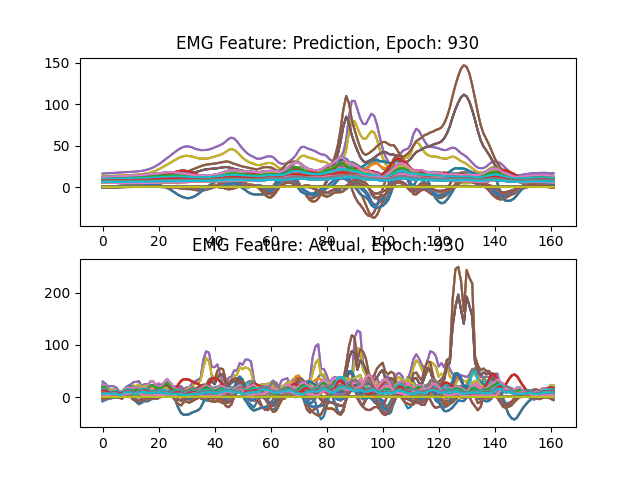
\includegraphics[width=0.75\linewidth]{graphics/emg_augment/real_vs_synth.png}
\end{figure}

\begin{figure}[hbtp]
    \caption{Mel Spectrogram from Transducer Trained with Real and Synthesized EMG}
    \label{fig:real-vs-pred-emg-3}
    \centering
    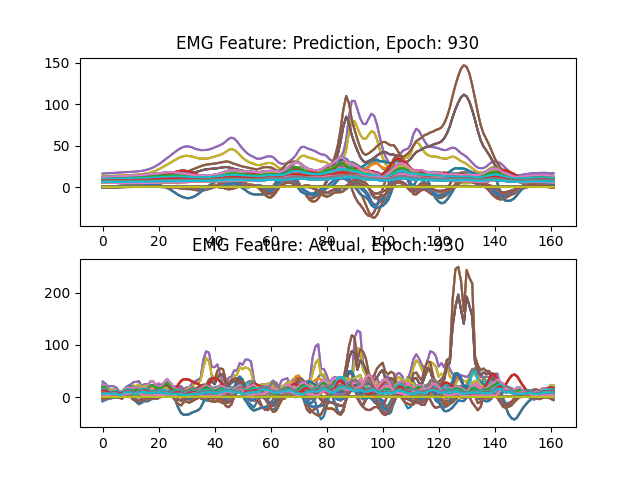
\includegraphics[width=0.75\linewidth]{graphics/emg_augment/real_vs_synth.png}
\end{figure}

As can be seen from the Figure \ref{gig:real-vs-pred-emg-2}, the EMG
synthesis model is able to learn the temporal relationship between
the input mel spectrograms and the target EMG signal. The synthesis
model is also able to learn the peaks of the EMG signals across time.
However, because the model is only learning a smoothed representation
of the underlying signal, it is not able to accuracy reproduce the EMG
signals which distinguish between different pitches. This can be seen
in Figure \ref{gig:real-vs-pred-emg-3}.

\subsection{Summary}

In summary, my hypothesis was disproved.
My initial hypothesis was that it was possible to simply reverse the
transduction network, which was introduced in the Digital Voicing paper
for transcribing from EMG features into speech features, but instead
reverse the features.

From my findings I found that this wasn't true because the low level 
features of the EMG data are difficult for the LSTM network to correctly
reproduce which hurts the models ability to accurately reproduce the
fine tuned parts of the EMG signal which correspond to the pitch of the
input signal.

In hindsight my approach could have been improved by being more selective in
the early stages. I could have determined which electrode contributed the most
in the transduction task, and then tried to just synthesise the signals for that 
particular channel and then tried to synthesise an increasing number of
electrode channels. I also could have used a convolutional layer
to generate the EMG signal.